%% LyX 2.2.4 created this file.  For more info, see http://www.lyx.org/.
%% Do not edit unless you really know what you are doing.
\documentclass[english]{article}
\usepackage[T1]{fontenc}
\usepackage[latin9]{inputenc}
\usepackage{geometry}
\geometry{verbose,lmargin=4.5cm,rmargin=4.5cm}
\usepackage{color}
\usepackage{babel}
\usepackage{verbatim}
\usepackage{float}
\usepackage{calc}
\usepackage{textcomp}
\usepackage{url}
\usepackage{graphicx}
\usepackage[unicode=true,pdfusetitle,
 bookmarks=true,bookmarksnumbered=false,bookmarksopen=false,
 breaklinks=true,pdfborder={0 0 1},backref=false,colorlinks=false]
 {hyperref}
\usepackage{breakurl}

\makeatletter
%%%%%%%%%%%%%%%%%%%%%%%%%%%%%% User specified LaTeX commands.
%\usepackage[T1]{fontenc}
\usepackage{charter}
\usepackage[table]{xcolor}
\usepackage{amsmath}
\newcommand{\mathA}[1]{{\operatorname{#1}}}
\newcommand{\mathB}[1]{{\operatorname{\mathit{#1}}}}


% Luis Garreta defs
\renewcommand{\textrightarrow}{$\rightarrow$}

\newcommand{\blue}[1]{{\textcolor{blue}{#1}}}

\usepackage[font=scriptsize,labelfont=bf]{caption}

%\pagecolor{yellow!30}

\makeatother

\usepackage{listings}
\renewcommand{\lstlistingname}{Listing}

\begin{document}

\title{MultiGWAS: A tool for GWAS analysis on tetraploid organisms by integrating
-four GWAS software}
\maketitle
\begin{abstract}
\textbf{Summary:} The Genome-Wide Association Studies (GWAS) are essential
to determine the association between genetic variants across individuals.
One way to support the results is by using different tools to validate
the reproducibility of the associations. Currently, software for GWAS
in diploids is well-established but for polyploids species is scarce.
Each GWAS software has its characteristics, which can cost time and
effort to use them successfully. Here, we present MultiGWAS, a tool
 perform GWAS analysis in tetraploid organisms by executing in parallel
and integrating the results from four existing GWAS  packages: two
available for polyploids (GWASpoly and SHEsis) and two frequently
used for diploids (PLINK and TASSEL). The tool deals with all the
elements of the GWAS process in the four packages, including (1) Genomica
data management from different input formats (2) Data cleaning using
different control quality filters, (3) Data conversion for package
file formats (4) GWAS Execution in the for packages using two GWAS
models, the full model with control for population structure and individual
relatedness and the Naive model without any control (5) Summary statististicswith
tables and plots describing intuitively the significant association
found by \textcolor{red}{both each one and across four packages,}
\textcolor{red}{which helps users to check for false-positive or false-negative
results.}
\end{abstract}

\section{Introduction}

%Ya est� modificada la intro para incluir diferentes especies de plantas poliploides. Faltan las citas. Estoy haciendo una lista de referencias que hay que leer con calma. Especialmente reviews. Intentar� en los pr�ximos d�as ampliarhttps://www.overleaf.com/project/5e8b8de6ae23ed0001a9a14f este primer p�rrafo conforme vaya leyendo las referencias que baj�. Pero el sentido general creo que ya qued� establecido. Att. Ivania 

The Genome-Wide Association Studies (GWAS) is used to identify which
variants through the whole genome of a large number of individuals
are associated with a specific trait (CITES). This methodology started
with humans and several model plants, such as rice, maize, and $Arabidopsis$
\cite{tian2011genome,korte2013advantages}. \textcolor{red}{Because
}of the advances in the next-gen sequencing technology and the decreasing
of the sequencing cost in recent years, there is an increase in genome
sequences in non-model organisms at a faster rate \cite{ekblom2011applications,ellegren2014genome}.
\textcolor{red}{Therefore}, several research projects pursue, for
the first time, the genetic bases of an ecological or economic phenotypic
variation through GWAS analysis for non-model wild plants and crops
that often are polyploids \cite{ekblom2011applications,santure2018wild}.

The GWAS for polyploid species has three related challenges.%
\begin{comment}
Me parece muy amplio este frase de los \emph{challeges}
\end{comment}
{} First, as all GWAS analyses, we should replicate the study as a reliable
method to validate the results and recognize real associations. This
replication involves finding the same associations either in an independent
population sample under the same software or using an independent
technology using the same population sample \cite{De2014,Pearson2008}.
Both approaches  involve the use of different parameters, models,
or conditions, to test how consistent the results are.

Second, although there are many GWAS packages available to repeat
the analysis under different conditions \cite{Gumpinger2018}, most
of them are designed exclusively for the diploid \textcolor{red}{data
matrix} \cite{Bourke2018}. Therefore, it is often necessary to \textquotedbl{}diploidizing\textquotedbl{}
the polyploid genomic data in order to replicate the analysis.

Third, the performance of different GWAS software could affect the
results. However, there are few tools focused in the integration of
the GWAS software outputs to make comparisons under different parameters
and conditions. For example, comparing four packages for diploid species
(i.e., PLINK, TASSEL, GAPIT, and FaST-LMM) using different sample
sizes for plant data found that the threshold $Pvalue$ for SNP significance
change for each package \cite{Yan2019}. It means that well-ranked
SNPs from one package can be ranked differently in another, causing
difficulty in selecting the most credible associations when results
from each package are analyzed separately. Besides, the software iPAT
facilitates the use of three popular command-line GWAS packages GAPIT,
PLINK, and FarmCPU \cite{Zhang2018}. However, results from the execution
of each package are separated. Therefore, the problem of interpreting
and selecting the best associations persists. In comparison, the easyGWAS
cloud platform, perform, share, and compare the results of GWAS \cite{Grimm2017}.
This platform offers two types of analysis: the first is an intersection
analysis that searches associations that were found significant in
more than one dataset. The second is a meta-analysis that searches
associations mutually supported by several datasets. Both types are
based on different datasets with the same GWAS parameters to confirm
or search for new associations. The limitation of this approach is
when the data set is unique or has a small sample of individuals.

To solve all the three challenges above, we developed the MultiGWAS
tool that performs GWAS analyses for tetraploid species using four
software in parallel. Our tool include GWASpoly \cite{Rosyara2016}
and the SHEsis tool \cite{Shen2016} that accept polyploid genomic
data, and PLINK \cite{Purcell2007} and TASSEL \cite{Bradbury2007}
with the use of a \textquotedbl{}diploidized\textquotedbl{} genomic
matrix. The tool deals with preprocessing data, running four GWAS
tools in parallel, and create reports that compare the results and
help the user decide more intuitively the true or false associations.

\section{Methods}

The MultiGWAS tool has three main consecutive steps: the adjustment,
the multi analysis, and finally, the integration (Fig. \ref{fig:Pipeline}).
In the adjustment step, MultiGWAS processes the configuration file,
cleans and filters the genotype and phenotype, and \textquotedbl{}diploidize\textquotedbl{}
the genomic data. Then, during the multi analysis, each GWAS tool
runs in parallel. Finally, in the integration step, the MultiGWAS
tool scans the output files from the four packages (i.e., GWASPoly,
SHEsis, PLink, and TASSEL). 

MultiGWAS generates a summary of all results that contains the following
tabular and graphical visualizations: score tables with detailed information
of associations, shared SNPs visualization using Venn diagrams, SNP
profiles using heatmaps, associations visualizations using Manhattan
and QQ plots, and chromosomes vs SNP visualizations using chord diagrams. 

% Figure MultiGWAS stages

\begin{figure}
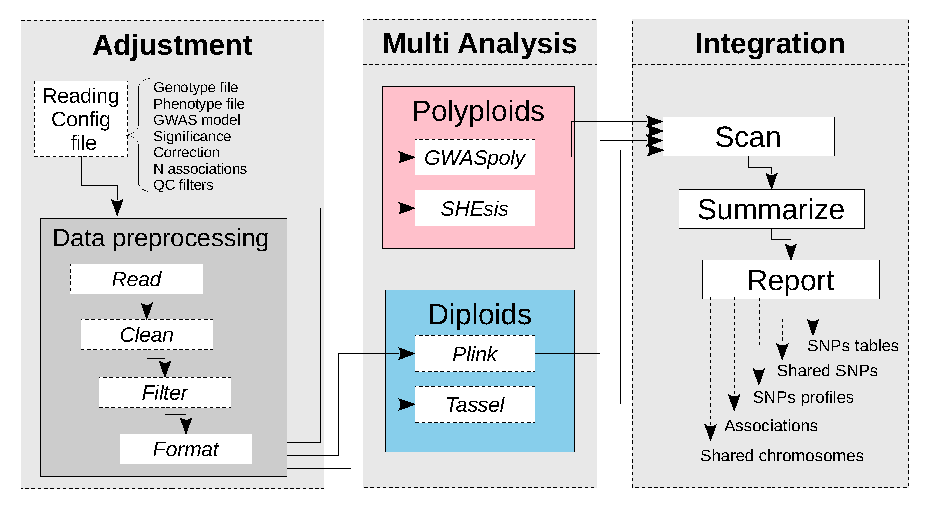
\includegraphics[width=12cm]{images/multiGWAS-flowchart-stages} \caption{MultiGWAS flowchart has three steps: adjustment, multi analysis, and
integration. The first step deals with input data management, reading
the configuration file and preprocessing the input genomic data (genotype
and phenotype). The second step deals with GWAS analysis, configuring
and running the four packages in parallel. And the third step deals
with summarizing and reporting results using different tabular and
graphical visualizations.\label{fig:Pipeline}}
\end{figure}


\subsection{Adjustment stage}

MultiGWAS takes as input a configuration file where the user specifies
the genomics data along with the parameters that will be used by the
four tools. Once the configuration file is read and processed, the
genomic data files (genotype and phenotype) are preprocessed by cleaning,
filtering, and checking data quality. The output of this stage corresponds
to the inputs for the four programs at the Multi Analysis stage.

%genotype/phenotype filenames, genome-wide significance threshold, multiple testing correction methods, GWAS model, number of associations to be reported, and TRUE or FALSE whether to use quality control (QC) filters or not. 

\subsubsection{Reading configuration file}

The configuration file includes the following settings that we briefly
describe:% (1) Input genotype and phenotype file names (2) GWAS model, (3) Significance threshold, (4) Correction (5) Quality Control (QC) filters and (6) number of associations to report. 

\paragraph{Input genotype and phenotype files:}

Currently, MultiGWAS uses two input files, one for genotype and the
other for the phenotype. Both data correspond to data matrices with
column and row names (Figure \ref{fig:File-Formats}). The genotype
file uses SNP markers in rows and samples in columns (Figure \ref{fig:File-Formats}a).
The phenotype file uses samples in rows and traits in columns (Figure
\ref{fig:File-Formats}b) with the first column corresponding to the
sample name and the second column to trait value.

%Paula: Luis una pregunta, recibimos solo formato ACGT? o recibimos otro formato?? 
% R/ Actualmente solo formato GWASpoly (dos archivos), se podría facilmente formato númerido, dos archivos (ClusterCall) con o sin info de mapa (CHROM, POSITION), y tal vez formato PLINK (tres archivos).

\begin{figure}[H]
\begin{centering}
\begin{minipage}[t]{0.6\columnwidth}%
\begin{center}
\fbox{\begin{minipage}[t]{0.99\columnwidth}%
\scriptsize\texttt{Marker,Chrom,Pos,Indiv01,Indiv02,Indiv03,...}

\texttt{c2\_41437,0,805179,AAAG,AAGG,AAGG,...}

\texttt{c2\_24258,0,1252430,AAGG,AGGG,GGGG,...}

\texttt{c2\_21332,0,3499519,TTCC,TTCC,TTCC,... }

\texttt{...}%
\end{minipage}}\\
a
\par\end{center}%
\end{minipage}~~~~~~~~~%
\begin{minipage}[t]{0.3\columnwidth}%
\begin{center}
\fbox{\begin{minipage}[t]{0.99\columnwidth}%
\scriptsize\texttt{Individual,Traitname}

\texttt{Indiv01, 3.59}

\texttt{Indiv02, 4.07}

\texttt{Indiv03, 1.05}

\texttt{...}%
\end{minipage}}\\
b
\par\end{center}%
\end{minipage}
\par\end{centering}
\begin{centering}
\par\end{centering}
\caption{\scriptsize \textbf{MultiGWAS genotype and phenotype formats}. Both
files are in CSV format (Comma Separated Values) and contain as first
row the header labels of the columns. Although the header labels are
arbitrary, the column order is obligatory. \textbf{a.} Genotype file
format, where ``Marker'', ``Chrom'', and ``Pos'', correspond
to the names for marker name, chromosome, and position in the first
three columns respectively. The next columns correspond to the columns
for the samples content. \textbf{b.} Phenotype file format, where
``Individual'' and ``Traitname'' are the column names for the
individual and trait names, respectively.\label{fig:File-Formats}}
\end{figure}


\paragraph{GWAS model:}

MultiGWAS is designed to work with quantitative phenotypes and can
run GWAS analysis using two types of statistical models that we have
called \emph{full} and \emph{naive} models. The \emph{full model}
is know in the literature as the Q+K model \cite{Yu2006} and includes
control for structure (Q) and relatedness between samples (K), whereas
the \emph{naive model} does not include any type of correction. Both
models are based on linear regression approaches and variations of
them are implemented by the four GWAS packages used by MultiGWAS.
The \emph{naive} is modeled with Generalized Linear Models (GLMs,
Phenotype + Genotype), and the \emph{full} is modeled with Mixed Linear
Models (MLMs, Phenotype + Genotype + Structure + Kinship). The default
model used by MultiGWAS is the \emph{full model} (Q+K) \cite{Yu2006},
which is expressed with the following equation:

\[
y=X\beta+S\alpha+Q\nu+Z\mu+e
\]

where $y$ is the vector of observed phenotypes; $\beta$ is a vector
of fixed effects other than SNP or population group effects; $\alpha$
is a vector of SNP effects (Quantitative Trait Nucleotides); $\nu$
is a vector of population effects; $\mu$ is a vector of polygene
background effects; $e$ is a vector of residual effects; $Q$, modeled
as a fixed effect, refers to the incidence matrix for subpopulation
covariates relating $y$ to $\nu$; and $X$, $S$ and $Z$ are incidence
matrices of 1s and 0s relating $y$ to $\beta$, $\alpha$ and $\mu$,
respectively.


\paragraph{Genome-wide significance: }

GWAS searches SNPs associated with the phenotype in a statistically
significant manner. A threshold or significance level $\alpha$ is
specified and compared with the \emph{p-value} derived for each association
score. Standard significance levels are 0.01 or 0.05 \cite{Gumpinger2018,Rosyara2016},
and MultiGWAS uses an $\alpha$ of 0.05 for the four GWAS packages.
But the threshold is adjusted according to each package, as some packages
as GWASpoly and TASSEL calculates the SNP effect for each genotypic
class using different gene action models (see ``Multi analysis stage'').
So, the number of tested markers\emph{ }may be different in each model
(see below) that results in different \emph{p-value} thresholds.

\paragraph{Multiple testing correction:}

Due to the massive number of statistical tests performed by GWAS,
it is necessary to perform a correction method for multiple hypothesis
testing and adjusting the \emph{p-value} threshold accordingly. Two
common methods for multiple hypothesis testing are the false discovery
rate (FDR) and the Bonferroni correction. The latter is the default
method used by MultiGWAS, which is one of the most stringent methods.
However, instead of adjusting the \emph{p-values,} MultiGWAS adjust
the threshold below which a \emph{p-value} is considered significant,
that is $\alpha/m$, where $\alpha$ is the significance level and
\emph{m }is the number of tested markers from the genotype matrix. 

\paragraph{Number of reported associations: }

Criticism has arisen in considering only statistically significant
associations as the only possible correct associations \cite{Thomson2011,Kaler2019}.
Many of low \emph{p-value} associations, closer to being significant,
are discarded due to the stringent significance levels, and consequently
increasing the number of false negatives. To help to analyze both
significant and non-significant associations, MultiGWAS provides the
option to specify the number of best-ranked associations (lower \emph{p-values}),
adding the corresponding \emph{p-value} to each association found.
In this way, it is possible to enlarge the number of results, and
we can observe replicability in the results for different programs.
Nevertheless, we present each association with the corresponding \emph{p-value}.

%  We present the resultant associations in different tables and graphics reported by MultiGWAS (see Figure \ref{fig:-View-Shared-SNPs}). 

\paragraph{Quality control filters:}

A control step is necessary to check the input data for genotype or
phenotype errors or poor quality that can lead to spurious GWAS results.
MultiGWAS provides the option to select and define thresholds for
the following filters that control the data quality: Minor Allele
Frequency (MAF), individual missing rate (MIND), SNP missing rate
(GENO), and Hardy-Weinberg threshold (HWE):
\begin{itemize}
\item \textbf{MAF of }\textbf{\emph{x:}} filters out SNPs with minor allele
frequency below \emph{x} (default 0.01); 
\item \textbf{MIND of }\textbf{\emph{x:}} filters out all individuals with
missing genotypes exceeding \emph{x}{*}100\% (default 0.1); 
\item \textbf{GENO of }\textbf{\emph{x:}} filters out SNPs with missing
values exceeding \emph{x}{*}100\% (default 0.1); 
\item \textbf{HWE of }\textbf{\emph{x:}} filters out SNPs which have Hardy-Weinberg
equilibrium exact test \emph{p-value} below the \emph{x} threshold.
\end{itemize}
MultiGWAS does the MAF filtering, and uses the PLINK package \cite{Gumpinger2018}
for the other three filters: MIND, GENO, and HWE. 

\subsubsection{Data preprocessing}

Once the configuration file is processed, the genomic data is read
and cleaned by selecting individuals present in both genotype and
phenotype. Then, individuals and SNPs with poor quality are removed
by considering the previous selected quality-control filters and their
thresholds, 

At this point, the format \textquotedbl{}ACGT\textquotedbl{} suitable
for the polyploid software GWASpoly and SHEsis, is \textquotedbl{}diploidized\textquotedbl{}
for PLINK and TASSEL. The homozygous tetraploid genotypes are converted
to diploid thus: AAAA\textrightarrow AA, CCCC\textrightarrow CC, GGGG\textrightarrow GG,
TTTT\textrightarrow TT. Moreover, for tetraploid heterozygous genotypes,
the conversion depends on the reference and alternate alleles calculated
for each position (e.g., AAAT\textrightarrow AT, ... ,CCCG\textrightarrow CG). 

After this process, the genomic data, genotype and phenotype, are
converted to the specific formats required for each of the four GWAS
packages.

\subsection{Multi analysis stage}

MultiGWAS runs in parallel using two types of statistical models specified
in the parameters file, the Full model (Q+K) and Naive (i.e., without
any control) \cite{Sharma2018}. The Full model (Q+K) controls for
both population structure and individual relatedness. For population
structure, MultiGWAS uses the Principal Component Analysis (PCA) and
takes the top \textcolor{blue}{five} PC as covariates. For relatedness,
\textcolor{blue}{MultiGWAS} uses kinship matrices that TASSEL and
GWASpoly calculated separately, and for PLINK and SHEsis, \textcolor{blue}{relatedness
depends of kinship coefficients calculated with the PLINK 2.0 built-in
algorithm \cite{Chang2015}. }

%\subsubsection{Tools}We have selected four GWAS software tools to
be integrated in our multiGWAS tool, two designed specifically for
polyploid species as many important crops are polyploids: GWASpoly
\cite{Rosyara2016} and SHEsis \cite{Yong2006}, and another two designed
for diploids species and extensively used in humans and plants: PLINK
\cite{Purcell2007,Chang2015} and TASSEL \cite{Bradbury2007}, respectively.

As MultiGWAS implements two types of GWAS analysis, naive and full,
each tool is called in two different ways. %The naive without any additional parameter, but the full with two parameters that take into account for population structure (Q) and relatedness (K) to prevent false associations.

\subsubsection{GWASpoly}

GWASpoly \cite{Rosyara2016} is an R package designed for GWAS in
polyploid species used in several studies in plants \cite{Berdugo2017,Ferrao2018,Sharma2018,Yuan2019}.
GWASpoly uses a Q+K linear mixed model with biallelic SNPs that account
for population structure and relatedness. \textcolor{blue}{Also, to
calculate the SNP effect for each genotypic class, GWASpoly provides
eight gene action models: general, additive, simplex dominant alternative,
simplex dominant reference, duplex dominant alternative, and duplex
dominant. As a consequence, the number of statistical test performed
can be different in each action model and so thresholds below which
the }\textcolor{blue}{\emph{p-values}}\textcolor{blue}{{} are considered
significant.}

MultiGWAS is using GWASpoly version 1.3, \textcolor{blue}{employing
all gene action models to find associations and repoting the top }\textcolor{blue}{\emph{N
}}\textcolor{blue}{best-ranked (the SNPs with lowest }\textcolor{blue}{\emph{p-values)}}\textcolor{blue}{,
where }\textcolor{blue}{\emph{N}}\textcolor{blue}{{} is defined by the
user in the input configuration file.} The \emph{full }model used
by GWASpoly includes the population structure and relatedness, which
are estimated using the first five principal components and the kinship
matrix, respectively, both calculated with the GWASpoly built-in algorithms.

\subsubsection{SHEsis}

SHEsis is another program designed for polyploid species that includes
single locus association analysis, among others. It is based on a
linear regresion model, and it has been used in some studies of animals
and humans \cite{Qiao2015,Meng2019}.

MultiGWAS is using the version 1.0 which does not take account for
population structure or relatedness, however MultiGWAS externally
estimates relatedness for SHEsis by excluding individuals with cryptic
first-degree relatedness using the algorithm implemented in PLINK
2.0 (see below).

\subsubsection{PLINK}

PLINK is one of the most extensively used programs for GWAS in diploids
species. It was developed for humans but it is applicable to any species
\cite{Power2016}. PLINK includes a range of analysis, including univariate
GWAS using two-sample tests and linear regression models.

MultiGWAS is using two versions of PLINK: 1.9 and 2.0. Linear regression
from PLINK 1.9 is used to achieve both types of analysis, naive and
full. For the full analysis, population structure is estimated using
the first five principal components calculated with the PLINK 1.9
built in algorithm. But relatedness is estimated from the kinship
coefficients calculated with the PLINK 2.0 built in algorithm, removing
the close relatives or individuals with first-degree relatedness.

\subsubsection{TASSEL}

TASSEL is another common GWAS program based on the Java software.
It was developed for maize and it has been used in several studies
in plants \cite{Alvarez2017,Zhang2018}, but like PLINK, it is applicable
to any species. For association analysis, TASSEL includes the general
lineal model (GLM) and mixed linear model (MLM) that accounts for
population structure and relatedness. \textcolor{blue}{And, in the
same manner that GWASPoly, TASSEL provides three gene action models
to calculate the SNP effect of each genotypc class: general, additive,
and dominant, and so the significance threshold depends of each action
model.}

MultiGWAS is using TASSEL 5.0, \textcolor{blue}{with all gene action
models used to find the }\textcolor{blue}{\emph{N }}\textcolor{blue}{best-ranked
associations and reporting the top }\textcolor{blue}{\emph{N }}\textcolor{blue}{best-ranked
associations (SNPs with lowest }\textcolor{blue}{\emph{p-values)}}\textcolor{blue}{.}
Naive GWAS is achieved by the GLM, and full GWAS is achieved by the
MLM with two parameters: population structure that uses the first
five principal components, and relatedness that uses the kinship matrix
with centered IBS method, both calculated with the TASSEL built-in
algorithms. 

\subsection{Integration stage.}

\color{blue}

The outputs resulting from the four GWAS packages are scanned and
processed to identify both significant and best-ranked associations
with \emph{p-values} lower than and close to a significance threshold,
respectively. 

\subsubsection{Calculation of \emph{p-values }and significance thresholds}

GWAS packages compute \emph{p-value }as a measure of association between
each individual SNP and the trait of interest. The SNPs are considered
statistically significant, and so possible true associations, when
their \emph{p-value }drops below a predefined significance threshold.
But, most GWAS packages compute differently \emph{p-values} with the
possibility to compute them too high or too low. If \emph{p-values}
are too high, then it would lead to false negatives or SNPs with true
associations with the phenotype but that does not reach the significance
threshold. Conversely, if \emph{p-values} are too low, then it would
lead to false positives or SNPs with false associations with the phenotype
but that reaches the significance threshold.

To overcome these difficulties, in the case of too high \emph{p-values},
MultiGWAS identifies and reports both significant and best-ranked
associations (the ones closer to being statistically significant).
Whereas, in the case of too low \emph{p-values}, MultiGWAS provides
two methods for adjusting \emph{p-values} and significance threshold:
the false discovery rate (FDR) that adjust \emph{p-values, }and the
Bonferroni correction, that adjusts the threshold.

By default, MultiGWAS uses the Bonferroni correction in which the
significance threshold is adjusted as $\alpha/m$, where $\alpha$
is the significance level defined by the user in the configuration
file, and $m$ is the number of tested markers in the GWAS study.
However, the significance threshold can be different for each GWAS
package as some of them use several action models to calculate the
SNP effect of each genotypic class. For both PLINK and SHEsis packages,
which use only one model, $m$ is equal to the total number of SNPs,
but for both GWASpoly and TASSEL packages, which use eight and three
gene action models, respectively, $m$ is equal to the number of test
performed in each model, which is different between models. 

\subsubsection{Selection of significant and best-ranked associations}

After corrections, significant associations are selected as the ones
with \emph{p-values} falling below a significant threshold, which
is calculated for each GWAS package. But, as described above, it is
equally important to know the best-ranked associations, closer to
being statistically significant, as they may represent important associations
to consider for posterior analysis. 

In the case of GWAS packages with only one gene action model (PLINK
and SHESIS), the best-ranked associations are selected from the top
\emph{N} identified by the package. But, in the case of GWAS packages
with several gene action models (GWASpoly and TASSEL), the best-ranked
associations are selected as the top \emph{N} from the ``best action
model'', the one with more shared SNP associations, in other words,
from the action model that identifies more associations that are also
identified in the other models.

\color{black}

\subsubsection{Integration of results}

% Figure several reports

\begin{figure}
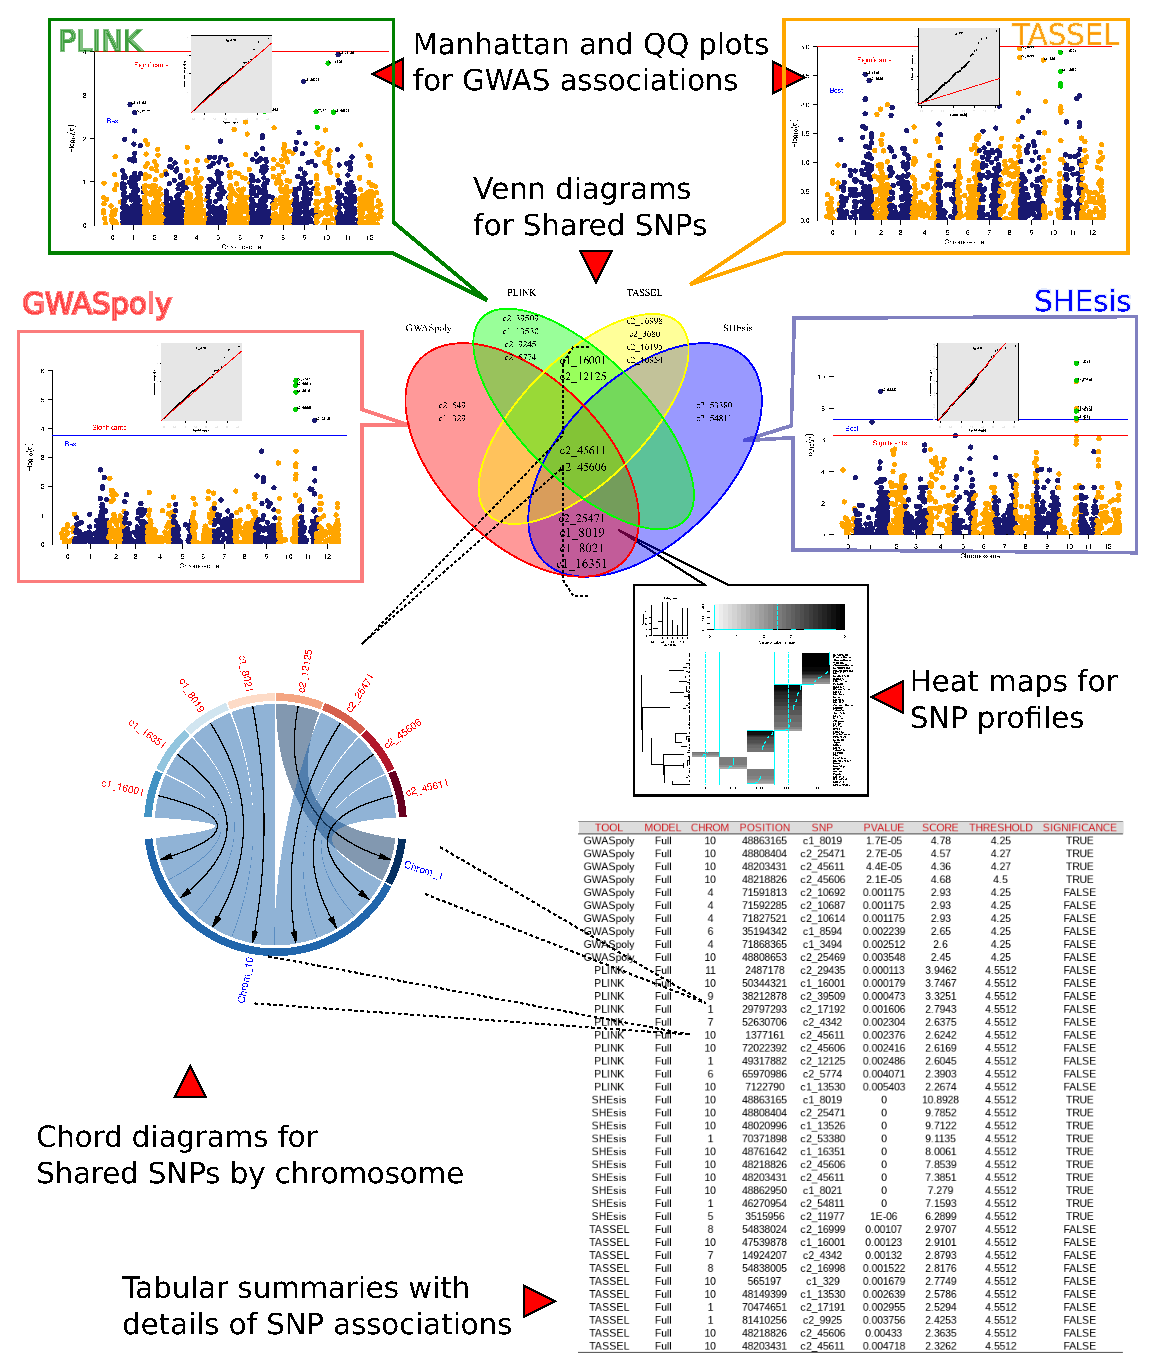
\includegraphics[width=12cm]{images/report-methodologies-all-plots}
\caption{\textbf{\textcolor{blue}{Reports presented by MultiGWAS}}\textcolor{blue}{.}
For each tool, first a QQ plot that \textcolor{blue}{assesses} the
resultant p-values. Second, a Manhattan plot for each tool with two
lines, blue and red, respectively, is the lower limit for the best
ranked and significative SNPs. We present two Venn diagrams, one for
the significative SNPs and one for N best-ranked SNPs of each tool.
We show the results for GWAspoly, PLINK, TASSEL, and SHEsis in red,
green, yellow, and blue, respectively. For each SNP that is in the
intersection; thus, that is predicted by more than one tool we provide
SNP profile. \textcolor{blue}{Chord diagrams for SNPs by chromosome
showing how the strongest associations are mostly found on few chromosomes.
And we also present tabular summaries with details of significant
and best-ranked associations. }\label{fig:Reports} }
\end{figure}

At this stage, \textcolor{blue}{MultiGWAS integrates} the results
to evaluate reproducible results among tools (Fig \ref{fig:Reports}).
But, it still reports a summary for the results of each tool: 
\begin{itemize}
\item A Quantile-Quantile (QQ) plots for the resultant \emph{p-values} of
each tool and the corresponding \textcolor{blue}{inflation factor}
$\lambda$ to asses the degree of the test statistic inflation. 
\item A Manhattan plot of each tool with two lower thresholds, one for the
best-ranked SNPs, and another for the significant SNPs. 
\end{itemize}
To present the replicability, we use two sets: (1) the set of all
the significative SNPs provided by each tool and (2) the set of all
the best-ranked SNPs. For each set, we present a Venn diagram that
shows SNPs predicted exclusively by one tool and intersections that
help to identify the SNPs predicted by one, two, three, or all the
tools. In addition, we provide detailed tables for the two sets.

For each SNP \textcolor{blue}{identified} more than once, we provide
what we call the SNP profile. That is a heat diagram for a specific
SNP, where each column is a genotype state AAAA, AAAB, AABB, ABBB,
\textcolor{blue}{and} BBBB. And each row corresponds to a sample.
Samples with close genotypes form together clusters. Thus to generate
the clusters, we do not use the phenotype information. However, we
present the phenotype information in the figure as the color. This
figure visually provides information regarding genotype and phenotype
information simultaneously for the whole population. We present colors
as tones between white and black for color blind people.

MultiGWAS generates a report, one document with the content previously
described. Besides, there is a folder with the individual figures
just in case the user needs one. In the supplementary information,
we include a report and a description of the report content\textcolor{red}{{}
(supplementary information XXX)}

%PAula: infomraciOn suplementary con reporte completo y figuras. Y explicaciOn del reporte

In the following section, we present the results applied to a public
dataset. 

\section{Results}

Most of the GWAS packages used by MultiGWAS are based on a linear
regression approaches, but they often produce dissimilar association
results for the same input. For example, computed \emph{p-values }for
the same set of SNPs are different between packages; SNPs with significant
\emph{p-values} for one package may be not significant for the others;
or well-ranked SNPs in one package may be ranked differently in another. 

To alleviate these difficulties, MultiGWAS produces five types of
outputs using different graphics and tabular views, these outputs
are intended to help users to compare, select, and interpret the set
of possible SNPs associated with a trait of interest. The outputs
include: 
\begin{itemize}
\item Manhattan and Q-Q plots to show GWAS associations. 
\item Venn diagrams to show associations identified by single or several
tools.
\item Heat diagrams to show the genotypic structure of shared SNPs.
\item Chord diagrams to show shared SNPs by chromosomes.
\item Score tables to show detailed information of associations for both
summary results from MultiGWAS and particular results from each GWAS
package
\end{itemize}
As an example of the functionality of the tool, here we show the outputs
reported by MultiGWAS in the tetraploid potato diversity panel, genotyped
and phenotyped as part of the USDA-NIFA Solanaceae Coordinated Agricultural
Project (SolCAP) \cite{Hirsch2013}. The complete report from MultiGWAS
for the naive and full model is in the Supplementary information (\url{https://github.com/agrosavia-bioinformatics/multiGWAS}) 


\subsection{Manhattan and QQ plots for GWAS associations }

MultiGWAS uses classical Manhattan and Quantile\textendash Quantile
plots (QQ plots) to visualize the results of GWAS analysis from each
package. In both plots, SNPs are represented by dots and their \emph{p-values}
are transformed to scores as $-log_{10}(\mathB{p-values})$ (see Figure
\ref{fig:view-qqmanhattan}). The Manhattan plot displays the SNP
association strength (y-axis) distributed in their genomic location
(x-axis), so the higher the score the stronger the association. Whereas
the QQ plot is used to visually compare the expected distribution
of \emph{p-values }(y-axis) vs. the observed distribution (x-axis),
so under the null hypothesis of no association of SNPs with the phenotype,
both distributions should coincide, and most SNPs should lie on a
diagonal line.

MultiGWAS adds special marks to the Manhattan and QQ plots to help
identify different types of SNPs: (a) In Manhattan plots, significant
SNPs are above a red line, best-ranked SNPs are above a blue line,
and shared SNPs (See Figure \ref{fig:Table-Shared-SNPs}.b) are colored
in green (b) In QQ plots, a red diagonal line indicates the expectation,
so potential associations can be observed when the number of SNPs
deviating from the diagonal is small, as in the case of monogenic
traits, or when this number is somewhat higher, as in the case of
truly polygenic traits. However, deviations for a high number of SNPs
could reflect inflated \emph{p-values }owing to population structure
or cryptic relatedness.

\begin{figure}[H]
\noindent %
\noindent\begin{minipage}[t]{1\columnwidth}%
\begin{center}
\includegraphics{images/paper-manhattan-QQ-plots}
\par\end{center}%
\end{minipage}

\caption{\textbf{MultiGWAS visualization of associations.} MultiGWAS creates
Manhattan and QQ plots for GWAS results of each GWAS packages. Here
we show the plots for one tetraploid package, GWASpoly (a), and other
diploid package, PLINK (b). \label{fig:view-qqmanhattan}}
\end{figure}


\subsection{Tables and Venn diagrams for single and shared SNPs}

MultiGWAS provides tabular and graphic views to report in an integrated
way both the best-ranked and significant SNPs identified by the four
GWAS packages (see Figure \ref{fig:Table-Shared-SNPs}). Both \emph{p-values}
and significance levels have been scaled as $-log_{10}(\mathB{p-value})$
to give high scores to the best statistically evaluated SNPs.

First, best-ranked SNPs correspond to the top-scored \emph{N} SNPs,
wheter they were assesed significant or not by its package, and with\emph{
N} defined by the user in the configuration file. These SNPs are shown
both in a SNPs table (Figure \ref{fig:Table-Shared-SNPs}.a) and in
a Venn diagram (Figure \ref{fig:Table-Shared-SNPs}.b). The table
lists them by package and sorts by decreasing score, whereas the Venn
diagram shows them emphasizing if they were best-ranked either in
a single package or in several at once (shared). And second, the significant
SNPs correspond to the ones assesed statistically significant by each
package, they are shown in a Venn diagram (Figure \ref{fig:Table-Shared-SNPs}.c),
and they are also shown in the SNPs table, marked with significance
TRUE (T) in the table of the Figure\ref{fig:Table-Shared-SNPs}.a.

\begin{figure}[H]
\begin{centering}
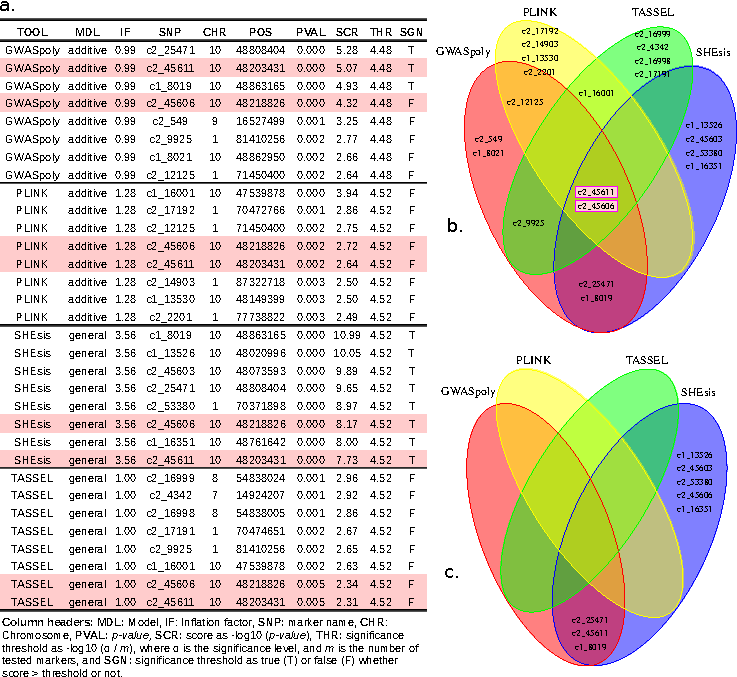
\includegraphics{images/paper-table-venn-best}
\par\end{centering}
\caption{\textbf{Shared SNPs Views. }Tabular and graphical views of SNP associations
identified by one or more GWAS packages (shared SNPs). SNPs identified
by all packages are marker with red background in all figures \textbf{(a)}
Table with details of the N=9 best-ranked SNPs from each GWAS package.
Each row corresponds to a single SNP and the 9 columns are: tool name,
model used by the tool, genomic control factor (inflation factor),
SNP name, chromosome, position in the genome, \emph{p-value}, score
as $-log_{10}(\mathB{p-value})$, significance threshold as $-log_{10}(\alpha/m)$
where $\alpha$ is the significance level and $m$ is the number of
tested markers, and significance as true (T) or false (F) whether
score > threshold or not. \textbf{(b)} Venn diagram of the N=9 best-ranked
SNPs. SNPs identified by all packages are located in the central intersection.
Other SNPs identified by more than one packages are located in both
upper central and lower central intersections. \textbf{(c)} Venn diagram
of the significant SNPs (score > threshold). \label{fig:Table-Shared-SNPs}}
\end{figure}

 

\subsection{Heat diagrams for structure of shared SNPs}

MultiGWAS creates a two-dimensional representation, called SNP profile,
to visualize each trait by individuals and genotypes as rows and columns,
respectively (Figure \ref{fig:SNP-profiles}). At the left, the individuals
are grouped in a dendrogram by their genotype. At the right, there
is the name or ID of each individual. At the bottom, the genotypes
are ordered from left to right, starting from the major to the minor
allele (i.e., AAAA, AAAB, AABB, ABBB, BBBB). At the top, there is
a description of the trait based on a histogram of frequency (top
left) and by an assigned color for each numerical phenotype value
using a grayscale (top right). Thus, each individual appears as a
colored line by its phenotype value on its genotype column. For each
column, there is a solid cyan line with the mean of each column and
a broken cyan line that indicates how far the cell deviates from the
mean.

Because each multiGWAS report shows one specific trait at a time,
the histogram and color key will remain the same for all the best-ranked
SNPs.

\begin{figure}[H]
\begin{centering}
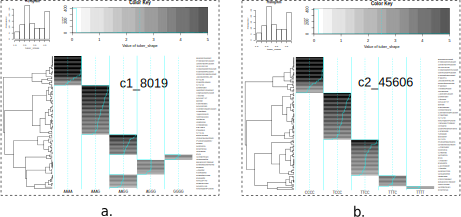
\includegraphics{images/paper-heat-maps}
\par\end{centering}
\caption{\textbf{\scriptsize{}SNP profiles. }{\scriptsize{}SNP profiles for
two of the best-ranked significant SNPs shown in the figure \ref{fig:Table-Shared-SNPs}.b.
(a) SNP c2\_45606 best-ranked by the four packages (central intersection
of the Venn diagram Figure \ref{fig:Table-Shared-SNPs}.b) (b) SNP
c1\_8019 best-ranked by the two tetraploid packages (Figure \ref{fig:Table-Shared-SNPs}.b),
and also identified as significant by the same packages (at the bottom
of the Figure \ref{fig:Table-Shared-SNPs}.a). \label{fig:SNP-profiles}}}
\end{figure}


\subsection{Chord diagrams for SNPs by chromosome}

Generally, in a typical GWAS analysis the strongest associations are
signaled by several nearby-correlated SNPs located in the same chromosome,
as in manhattan plots, where these associations form neat peaks with
several SNPs showing the same signal. Conversely, no peaks are shown
when few SNPs correlate with a trait. 

However, when the analysis is performed by several GWAS packages,
as MultiGWAS does, it can identify correlated SNPs between packages
that show the same signal, what is presented by MultiGWAS through
chord diagrams. For exampele, the Figure \ref{fig:Chord-diagrams}.a
shows the chord diagram for the shared SNPs from the best-ranked associations
previously described in the Figure \ref{fig:Table-Shared-SNPs}.b.
It can be observed that most SNPs relate to chromosome 10 and only
one to chromosome 1, which is also observed in the manhattan plots
from each GWAS package (Figure \ref{fig:Chord-diagrams}.b).

\begin{figure}
\begin{centering}
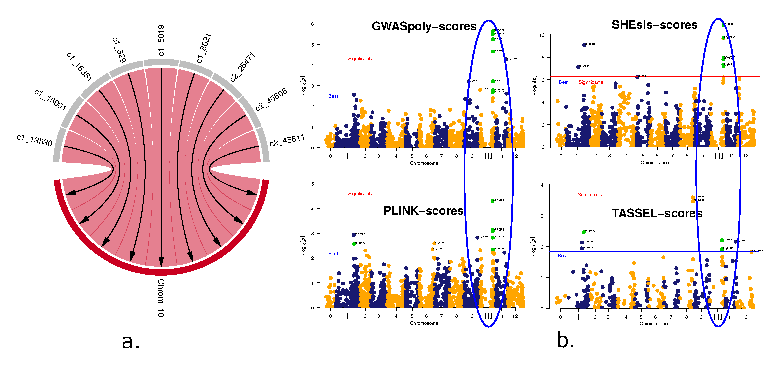
\includegraphics{images/paper-chord-manhattans}
\par\end{centering}
\caption{\textbf{SNPs by chromosome.} The figure shows how the best-ranked
SNPs relate to chromosomes. \textbf{(a)} Chord diagram showing that
most SNPs related to chromosome 10. SNPs are at the top of the diagram,
chromosomes at the botton, and associations are represented by arrows
drawn from SNPs to their chromosomes. The more associations identified
in one chromosome, the wider the space of its sector. \textbf{(b)}
Manhattan plots from each GWAS packages showing two important locations
of associations: chromosome 1 and chromosome 10, marked with a blue
and red ellipsis, respectively. \label{fig:Chord-diagrams}}

\end{figure}


\section{Availability and Implementation}

The core of the MultiGWAS tool was developed in R and users can interact
with the tool by either a command line interface (CLI) developed in
R or a graphical user interface (GUI) developed in Java (Figure \ref{fig:MultiGWAS-interaction}).
Source code, examples, documentation and installation instructions
are available at \url{https://github.com/agrosavia-bioinformatics/multiGWAS}. 

\subsection{Input parameters}

MutiGWAS uses as the only input a simple configuration text file where
users set the values for the main parameters that drives the GWAS
process. The file can be created either using a general text editor
or using the MultiGWAS GUI application (see below). In both cases,
the file must have the structure shown in the Figure \ref{fig:Configuration-file}.a,
where parameter names and values are separated by colon, filenames
are enclosed in quotation marks, and TRUE or FALSE indicates wheter
filters are applied or not. In the second case, the user creates the
config file in a simple and straightforward way using the input parameter
view from the GUI application (see below).

\begin{figure}[H]
\begin{centering}
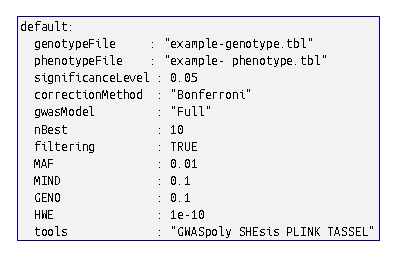
\includegraphics{images/paper-config-file}
\par\end{centering}
\caption{Configuration file for MultiGWAS. The input parameters include: the
output folder where results will be written, input genotype/phenotype
filenames, genome-wide significance threshold, method for multiple
testing correction, GWAS model, number of associations to be reported,
filtering with TRUE or FALSE whether to use quality control filters
or not. The filters are: minor allele frequency, individual missing
rate, SNP missing rate, and Hardy-Weinberg threshold. At the end the
tools parameter defines the GWAS packages to be used for the analysis.
\label{fig:Configuration-file}}
\end{figure}


\subsection{Using the command line interface}

The execution of the CLI tool is simple, it only needs to open a
linux console, change to the folder where the configuration file was
created, and type the name of the executable tool followed by the
filename of the configuration file, like this:

\begin{lstlisting}[language=bash,basicstyle={\small}]
multiGWAS Test01.config
\end{lstlisting}

Then, the tool starts the execution, showing information of the process
in the console window, and when it finishes the results are saved
to a new subfolder called \emph{``out-Test01}. Results include a
full html report containing the different views described in the results
section, along with the original graphics and summary tables created
by MultiGWAS and used to create the html report. Additionally, results
include the preprocessed tables of the main outputs generated by the
four GWAS packages used by MultiGWAS.

\subsection{Using the graphical user interface}

The MultiGWAS GUI can be executed by calling from a linux console
the following command:

\begin{lstlisting}[language=bash,basicstyle={\small}]
jmultiGWAS
\end{lstlisting}

After it opens, it shows a main frame with a tool bar at left and
four tabs at the top (Figure \ref{fig:MultiGWAS-interaction}). From
the tool bar, users can select the GWAS packages to use in the analysis\textendash two
for tetraploids and two for diploids\textendash , and start the analysis
with the current parameters (or with parameters from a previous configuration).
And, from the tabs, users can input the MultiGWAS parameters, and
view the process and results of the analysis.

.

\begin{figure}[H]
\begin{centering}
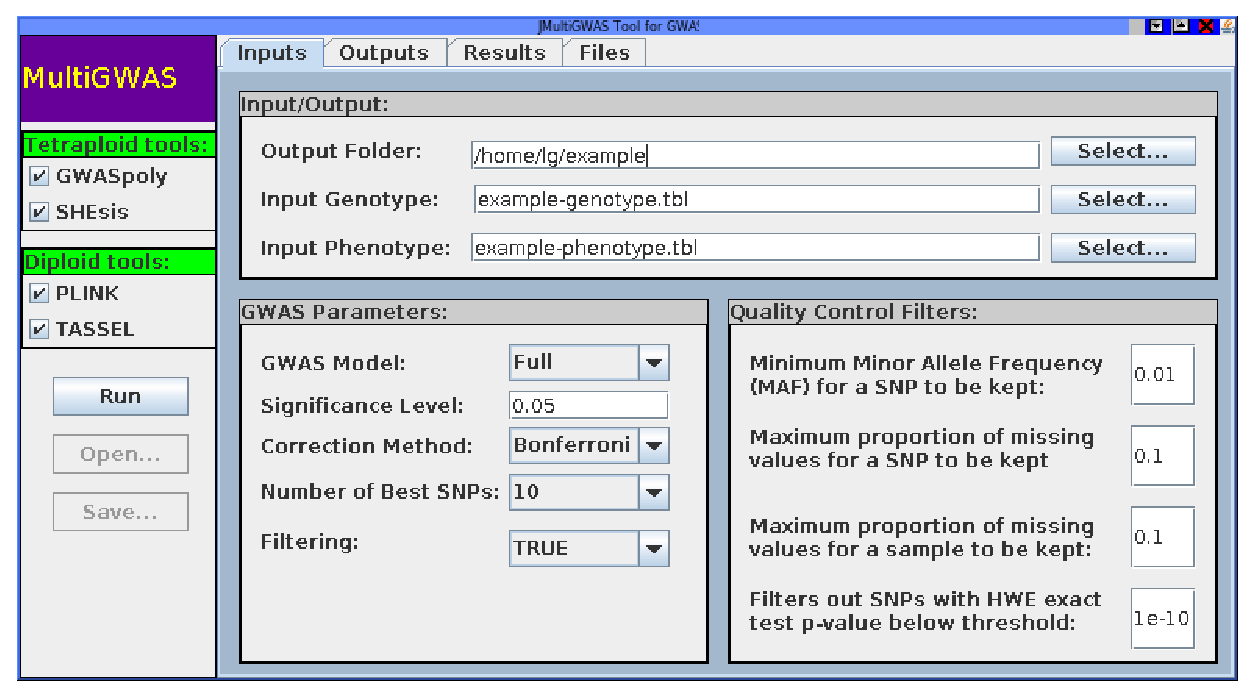
\includegraphics[scale=0.5]{images/paper-implementation-jmultiGWAS}
\par\end{centering}
\caption{\scriptsize\textbf{MultiGWAS GUI application}. Main view of the MultiGWAS
GUI application (``Inputs'' view) where users can create the configuration
file by setting values for input parameters. The GUI contains other
three views: ``Outputs'' view shows the logs of the running process.
``Results'' view shows a report in html format with the tabular
and graphics described in the results section. And, the ``Files''
view shows an embedded file manager pointing to the subfolder that
contains the files created by MultiGWAS and used to create the report.
\protect \\
\label{fig:MultiGWAS-interaction}}
\end{figure}

\bibliographystyle{plain}
\bibliography{multiGWAS}

\end{document}
